\documentclass[10pt, a5paper]{article}
\usepackage{pdfpages}
\usepackage{parallel}
\usepackage[T2A]{fontenc}
\usepackage{ucs}
\usepackage[utf8x]{inputenc}
\usepackage[polish,english,russian]{babel}
\usepackage{hyperref}
\usepackage{rotating}
\usepackage[inner=2cm,top=1.8cm,outer=2cm,bottom=2.3cm,nohead]{geometry}
\usepackage{listings}
\usepackage{graphicx}
\usepackage{wrapfig}
\usepackage{longtable}
\usepackage{indentfirst}
\usepackage{array}
\newcolumntype{P}[1]{>{\raggedright\arraybackslash}p{#1}}
\frenchspacing
\usepackage{fixltx2e} %text sub- and superscripts
\usepackage{icomma} % коскі ў матэматычным рэжыме
\PreloadUnicodePage{4}

\newcommand{\longpage}{\enlargethispage{\baselineskip}}
\newcommand{\shortpage}{\enlargethispage{-\baselineskip}}

\def\switchlang#1{\expandafter\csname switchlang#1\endcsname}
\def\switchlangbe{
\let\saverefname=\refname%
\def\refname{Літаратура}%
\def\figurename{Іл.}%
}
\def\switchlangen{
\let\saverefname=\refname%
\def\refname{References}%
\def\figurename{Fig.}%
}
\def\switchlangru{
\let\saverefname=\refname%
\let\savefigurename=\figurename%
\def\refname{Литература}%
\def\figurename{Рис.}%
}

\hyphenation{admi-ni-stra-tive}
\hyphenation{ex-pe-ri-ence}
\hyphenation{fle-xi-bi-li-ty}
\hyphenation{Py-thon}
\hyphenation{ma-the-ma-ti-cal}
\hyphenation{re-ported}
\hyphenation{imp-le-menta-tions}
\hyphenation{pro-vides}
\hyphenation{en-gi-neering}
\hyphenation{com-pa-ti-bi-li-ty}
\hyphenation{im-pos-sible}
\hyphenation{desk-top}
\hyphenation{elec-tro-nic}
\hyphenation{com-pa-ny}
\hyphenation{de-ve-lop-ment}
\hyphenation{de-ve-loping}
\hyphenation{de-ve-lop}
\hyphenation{da-ta-ba-se}
\hyphenation{plat-forms}
\hyphenation{or-ga-ni-za-tion}
\hyphenation{pro-gramming}
\hyphenation{in-stru-ments}
\hyphenation{Li-nux}
\hyphenation{sour-ce}
\hyphenation{en-vi-ron-ment}
\hyphenation{Te-le-pathy}
\hyphenation{Li-nux-ov-ka}
\hyphenation{Open-BSD}
\hyphenation{Free-BSD}
\hyphenation{men-ti-on-ed}
\hyphenation{app-li-ca-tion}

\def\progref!#1!{\texttt{#1}}
\renewcommand{\arraystretch}{2} %Іначай формулы ў матрыцы зліпаюцца з лініямі
\usepackage{array}

\def\interview #1 (#2), #3, #4, #5\par{

\section[#1, #3, #4]{#1 -- #3, #4}
\def\qname{LVEE}
\def\aname{#1}
\def\q ##1\par{{\noindent \bf \qname: ##1 }\par}
\def\a{{\noindent \bf \aname: } \def\qname{L}\def\aname{#2}}
}

\def\interview* #1 (#2), #3, #4, #5\par{

\section*{#1\\{\small\rm #3, #4. #5}}

\def\qname{LVEE}
\def\aname{#1}
\def\q ##1\par{{\noindent \bf \qname: ##1 }\par}
\def\a{{\noindent \bf \aname: } \def\qname{L}\def\aname{#2}}
}


\begin{document}
\renewcommand{\figurename}{Рыс.} % Не перакідаць у прэамбулу --- не працуе, чаму -- халера ведае.
\renewcommand{\abstractname}{Анатацыя}
\renewcommand{\refname}{Літаратура}

\title{Выкарыстанне свабоднага праграмнага забеспячэння ва ўстановах адукацыі Украіны: спроба аналізу}

\author{Грыгорый Злобiн\\
\small Львоўскі нацыянальны ўніверсітэт ім. Івана Франка,\\
\small \texttt{zlobin@electronics.wups.lviv.ua}
}
\date{}

\maketitle

\begin{abstract}
The analysis of free / open source software usage in higher educational institutions of Ukraine is presented, based of the ``FOSS Lviv-2011''  International Scientific Conference reports. 
\end{abstract}

Нягледзячы на станоўчы досвед выкарыстання свабодных праграм у адукацыі як у краінах блізкага, так і далёкага замежжа, ва Украіне да гэтага часу не прынятая канцэпцыя выкарыстання свабоднага праграмнага забеспячэння у адукацыі. Разам з тым намаганнямі энтузіястаў у навучальных установах Украіны свабоднае праграмнае забеспячэнне ўсё ж выкарыстоўваецца! Праз адасобленую пазіцыю Міністэрства адукацыі і навукі Украіны няма падрабязнай інфармацыі аб досведзе выкарыстання свабодных праграм у адукацыі. Дзякуючы таму, што ў Львоўскім нацыянальным універсітэце імя Івана Франка 01--06 лютага 2011 адбылася даволі прадстаўнічая міжнародная навукова"=практычная канферэнцыя <<FOSS Lviv-2011>>, з'явілася магчымасць правядзення аналізу выкарыстання СПЗ у вышэйшых навучальных установах Украіны. З 81 дакладаў 49 было прысвечана выкарыстанню СПЗ у навучальных установах. Даклады \cite{fosslviv}, якія былі пададзеныя на гэтую канферэнцыю, можна згрупаваць па наступных кірунках (назва дакладу падаецца на мове арыгіналу):

\section*{Дыстанцыйнае навучанне}
Гэтай тэматыцы прысвечаная найбольшая колькасць дакладаў "--- 10:
\begin{itemize}
\item <<Розроблення електронного деканату для системи управління дистанційним навчання MOODLE>> --- Артеменко В.Б., Львоўская камерцыйная акадэмія
\item <<Вибір платформи дистанційного навчання>> --- Коцаренко М.В., Бойко О.В.,  Львоўскі нацыянальны медыцынскі ўніверсітэт ім. Данііла Галіцкага
\item <<Використання контрольно-діагностичної програми iTest у ході моніторингу якості процесу навчання старшокласників>> --- Макаренко І.Є., Мерзлікін П.В., Крыварожскі дзяржаўны педагагічны ўніверсітэт
\item  <<Використання системи Moodle для організації контролю знань майбутніми вчителями-гуманітаріями>> --- Маркова Є.С., Бердзянскі дзяржаўны педагагічны ўніверсітэт
\item  <<Тестування в  Moodle як елемент менеджменту якості освіти: перший досвід>> --- Сергієнко В.П., Сліпухіна І.А., НПУ ім. М.П. Драгаманава
\item  <<Особливості програмного забезпечення в електронному навчанні>> --- Жарких Ю.С., Лисоченко С.В., Сусь Б.Б., Третяк О.В., Кіеўскі нацыянальны ўніверсітэт ім. Тараса Шаўчэнкі
\item  <<Інформаційно-аналітична система управління навчальним процесом ВНЗ на базі  Moodle>> --- Триус Ю.В., Чаркаскі дзяржаўны тэхналагічны ўніверсітэт
\item  <<Використання CMS JOMLA!  та LCMS MOODLE у ВНЗ>> --- Франчук В.М., НПУ ім. М.П. Драгаманава
\item <<Локалізація системи MOODLE " --- Франчук В.М., НПУ ім. М.П. Драгаманава
\item  <<Застосування вільного програмного забезпечення для дистанційного навчання у вищих навчальних закладах>> --- Захарченко В.М., Шапо В.М., Адэская нацыянальная марская акадэмія
\end{itemize}
\newpage

\section*{Выкарыстанне сістэм кампутарнай матэматыкі}
Наступныя 6 дакладаў можна аднесці да матэматычнай тэматыкі:
\begin{itemize}
\item <<Використання вільно-поширюваного ПЗ математичного призначення в університеті>> "--- Бугаєць Н.О., НПУ ім. М.П. Драгаманава
\item <<Вільнопоширювані системи комп'ютерної математики в осві\-ті і науці>> "--- Лазурчак І.І., Кобильник Т.П., Драгобыцкі дзяржаўны ўніверсітэт ім. І. Франка
\item <<Використання комп'ютерних математичних систем у про\-фе\-сій\-ній підготовці майбутнього вчителя математики>> "--- Лов'я\-но\-ва І.В., Крыварожскі дзяржаўны педагагічны ўніверсітэт
\item <<Моделювання задач електротехніки у XCOS>> "--- Філь І.М., Данецкі нацыянальны тэхнічны ўніверсітэт
\item <<Розробка і використання web-інтерфейсів для роботи з системами комп'ютерної математики>> "--- Чичкарьов Є.А., Прыазоўскі дзяржаўны тэхнічны ўніверсітэт
\item <<Про комп'ютерний супровід викладання геометрії>> "--- Яхненко І.В., Лутфулін М.В., Палтаўскі нацыянальны педагагічны ўніверсітэт ім. В.Г. Караленкі
\end{itemize}

\section*{Агульныя пытанні выкарыстання СПЗ у адукацыі}
7 дакладаў гэтай групы, якую можна прызнаць другой па колькасці, уключалі:
\begin{itemize}
\item <<Використання вільного програмного забезпечення в навчанні і наукових дослідженнях у Львівському національному уні\-вер\-ситеті імені Івана Франка>> "--- Апуневич С.Є., Злобін Г.Г., Рикалюк Р.Є., Шувар Р.Я., Львоўскі нацыянальны ўніверсітэт ім. І. Франка
\item <<Використання вільного програмного забезпечення в системі дистанційної освіти>> "--- Воронкін О.С., Луганскі дзяржаўны інстытут культуры і мастацтваў
\item <<Вільнопоширюване програмне забезпечення курсу “Нові інформаційні технології” для студентів спеціальності \linebreak “Біо\-ло\-гія”>> "--- Єфименко В.В., НПУ ім. М.П. Драгаманава
\item <<Використання вільного програмного забез\-печення у про\-фе\-сій\-ній підготовці майбутніх інженерів>> "--- Покришень Д.А., \linebreak Дрозд О.П., Сподаренко І.Й., Чарнігаўскі дзяржаўны тэхналагічны ўніверсітэт
\item  <<Про досвід використання ОС Linux у навчальному процесі Львівського національного медичного університету імені Данила Галицького>> "--- Риковський П.А., Львоўскі нацыянальны медыцынскі ўніверсітэт ім. Данііла Галіцкага
\item  <<LINUX  та VIRTUAL-BOX у навчанні абстрактних понять теорії операційних систем>> "--- Спірін О.М., Сверчевська О.С., Жытомірскі дзяржаўны ўніверсітэт ім. І. Франка
\item  <<З досвіду використання вільного програмного забезпечення при вивченні інформатики>> "--- Харченко В.М., Нежынскі дзяржаўны ўніверсітэт ім. М. Гогаля
\end{itemize}

\section*{Выкарыстанне адкрытых сродкаў праграмавання}
Гэтая група апынулася найменшай па колькасці і ўключае 4 даклады:
\begin{itemize}
\item <<Використання відкритих програмних засобів в процесі навчання статистичним дисциплінам>> "--- Коркуна Т.Й., Самбарскі тэхнікум эканомікі і інфарматыкі
\item <<Розрахунок фотоіонізаційних моделей небулярного газу в ОС LINUX UBUNTU 10.10 та WINDOWS 7>> "--- Мелех Б.Я., Тишко Н.Л., Коритко Р.І., Львоўскі нацыянальны ўніверсітэт ім. І. Франка
\item <<Реалізація розподілених обчислень на основі грід-платформи з відкритим кодом BOINC>> "--- Шийка Ю.Я., Шувар Р.Я., \linebreak Львоўскі нацыянальны ўніверсітэт ім. І. Франка
\item <<Реалізація високопродуктивної обчислювальної системи на базі ОС  LINUX>> "--- Шувар Р.Я., Бойко Я.В., Львоўскі нацыянальны ўніверсітэт ім. І. Франка
\end{itemize}

\section*{Распрацоўка праграмнага забеспячэння}
Будучы тэматычна-роднаснай папярэдняй, гэтая група больш шматлікая і складаецца з 7 дакладаў, яна зраўнавалася з катэгорыяй <<Агульныя пытанні выкарыстання СПЗ у адукацыі>>:
\begin{itemize}
\item <<Комплекс програм для лазерних спостережень штучних супутників Землі>> "--- Мартинюк-Лотоцький К.П., Білінський\linebreak А.\,І., Львоўскі нацыянальны ўніверсітэт ім. І. Франка
\item <<Розробка системи спектральної діагностики димової плазми>> "--- Сподарець Д.В., Драган Г.С., Адэскі нацыянальны ўні\-версітэт імя І.І. Мечнікава
\item <<Використання вільного програмного забез-печення для створення програми керування інформаційним автоматом>> "--- Зло\-бін Г., Скляр В., Чмихало О., Шевчик В., Львоўскі нацыянальны ўніверсітэт ім. І. Франка
\item <<Використання бібліотеки класів GEANT4 в ОС Linux при розробці програмного забезпечення для моделювання процесів взаємодії випромінювання з речовиною>> "--- Малихіна Т.В., Харкаўскі нацыянальны ўніверсітэт ім. В.Н. Каразіна
\item  <<Програма для обробкирезультатів ЛЛС-спостережень як \linebreak ВПЗ>> "--- Апуневич С.Є., Апуневич С.В., Білінський А.І., Благодир Я.Т., Львоўскі нацыянальны ўніверсітэт ім. І. Франка
\item  <<Програмне забезпечення керування телескопом  ЛЛС-станції Львів-1831>> "--- Білінський А.І., Мартинюк-Лотоцький К.\,П., \linebreak Львоўскі нацыянальны ўніверсітэт ім. І. Франка
\item <<Використання Open Wrt як основи вбудованого програмного забезпечення маршрутизаторів>> "--- Нек Т., Львоўскі нацыянальны ўніверсітэт ім. І. Франка
\end{itemize}

\section*{Асобныя даклады}
І нарэшце, 5 дакладаў немагчыма аднесці ні да адной з пералічаных вышэй катэгорый:
\begin{itemize}
\item  <<Інформаційна технологія управління навчальним навантаженням у вищих навчальних закладах>> "--- Гриценко В.Г., Чаркаскі нацыянальны ўніверсітэт ім. Б. Хмяльніцкага
\item  <<Про досвід використання офісного  пакету OpenOffice.org.ukr в курсі інформатики для економічних і юридичних спеціальностей ВЗО>> "--- Злобін Г.Г., Львоўскі нацыянальны ўніверсітэт ім. І. Франка 
\item  <<Досвід використання  редактора Gimp при вивченні курсу “Комп'ютерна графіка і дизайн”>> "--- Матвієнко Ю.С., Палтаўскі нацыянальны педагагічны ўніверсітэт ім. В.Г. Караленкі
\item <<Використання програми GANTTPROJECT для побудови календарних графіків при розробці ПВР>> "--- Грицук Ю.В., Меліхов О.І., Данбаская акадэмія будаўніцтва і архітэктуры
\item <<Вільне ПЗ для підготовки наукових текстів і презентацій>> "--- Лутфуллін М.В., Моторний М.І., Палтаўскі нацыянальны педагагічны ўніверсітэт ім. В.Г. Караленкі
\end{itemize}

	Такім чынам, можна канстатаваць як шырокі спектр выкарыстання СПЗ ва ўкраінскіх навучальных установах ад дыстанцыйнага навучання да распрацоўкі адкрытага праграмнага забеспячэння, так і шырокую геаграфію выкарыстання СПЗ ад Луганска на ўсходзе да Львова на захадзе і ад Чарнігава на поўначы да Адэсы на поўдні (глядзі рыс.).

\begin{figure}[ht]
\centering{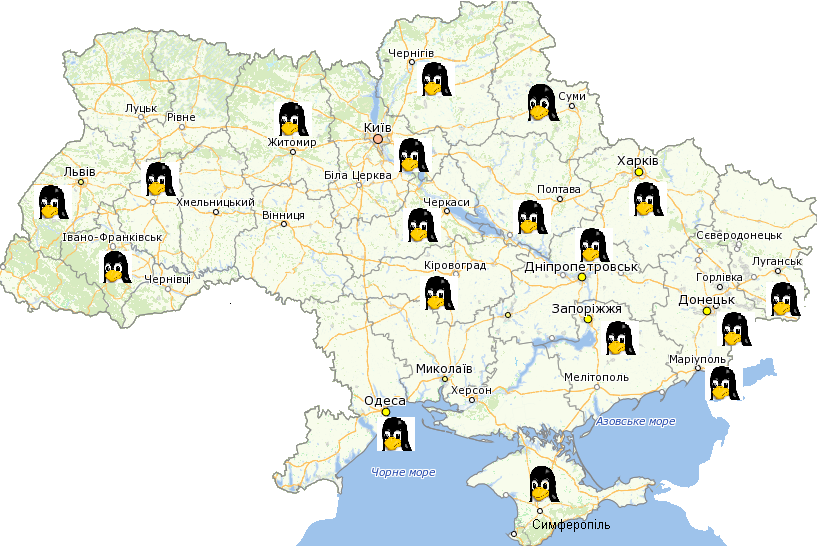
\includegraphics[width=8cm]{05_ukraine_linux.png}}
\label{pic:fl1}
%\caption{~}
\end{figure}

\begin{thebibliography}{9}
\bibitem{fosslviv}Тези міжнародної науково-практичної конференції FOSS LVIV-2011. Збірник наукових праць /за ред. Злобіна Г.Г., Апуневича С.Є., Машкова В.В., Апуневич С.В. Вид-во ЛНУ імені Івана Франка. 2011. --- 196 с.
\end{thebibliography}

\end{document}




